 \documentclass[a4paper,10pt]{article}
\input{/Users/WannaGetHigh/workspace/latex/macros.tex}

\title{Rapport TP HCM, PCM, Dav\'e}
\author{Fran\c cois \bsc{Lepan}}

\begin{document}
\maketitle

\section*{Introduction}

Dans le TP pr\'ec\'edent nous avons vu comment faire pour segmenter une image via la m\'ethode FCM (Fuzzy C-Means). Nous allons maintenant voir trois autres m\'ethodes Hard C-Means (HCM), Possibilistic C-Means (PCM) et Dav\'e. \\

Voici un rapel de la Methode FCM.

\begin{paragraph}{Initialisation}~\\

Pour commencer cette m\'ethode \`a besoin du nombre de cluster (classe). Avec ce nombre on initialise les centro\?ides al\'eatoirement  (non supervis\'e) ou en les s\'electionnant manuellement (supervis\'e).

On stock chaque pixel dans une matrice $3*nombreDePixel$ : 3 pour l'espace RGB.

Ensuite on initialise une matrice de distance entre les pixels et les centro\?ides. Gr�ce \`a cette matrice on va en d\'eduire le degr\'e d'appartenance (comprit entre 0 et 1) des pixels par rapport a tous les cluster.
\end{paragraph}

\begin{paragraph}{Boucle principale}~\\

On va r\'ep\'eter n fois ces op\'erations, n \'etant demander \`a la base.

\begin{itemize}
\item on recalcule tout d'abord la position des centres des clusters d'apr\`es les distances et les degr\'es d'appartenance calcul\'es lors du tour pr\'ec\'edent.
\item on recalcule la distance de chaque pixel \`a ces nouveaux centres ainsi que leur degr\'e d'appartenance \`a chaque cluster.
\item on calcule la performance de l'algo.
\end{itemize}
\end{paragraph}
~\\

Les trois m\'ethodes qui suivent se base sur le m\^eme proc\'ed\'e \`a quelques diff\'erences pr\`es. Les r\'esultats pr\'esent\'e se base sur la Fig.\ref{img_de_base} et utilise une m\'ethode supervis\'e.

\begin{figure}[ht]
\begin{center}
	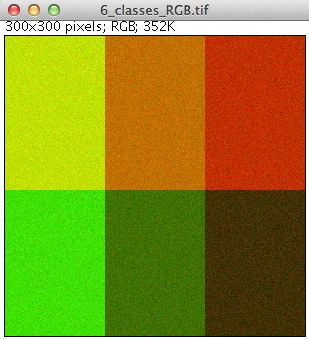
\includegraphics[width=5cm]{images/img_de_base.png}
\end{center}
	\caption{Image utilis\'e}
	\label{img_de_base}
\end{figure}

\newpage

\section{Hard C-Means}

Pour HCM le premier changement se fait lors du calcule du degr\'e d'appartenance. On ne donne plus une valeur entre z\'ero et un pour un pixel donn\'e, on force la classe en mettant 0 partout et 1 pour la classe qui est la plus proche. Ensuite le sons changement se fait sur la valeur de flou qui doit \^etre fix\'e \`a 1.

\begin{figure}[ht]
\begin{center}
	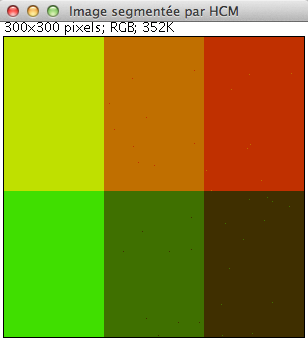
\includegraphics[width=5cm]{images/hcm_img_sup}
	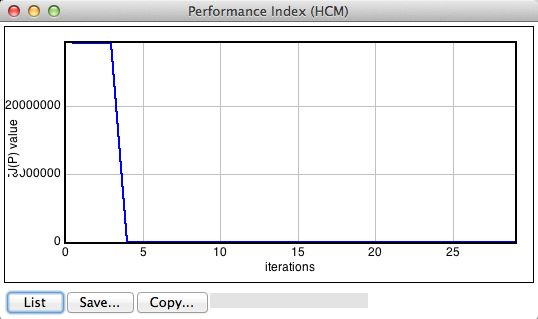
\includegraphics[width=9cm]{images/hcm_courbe_sup}
\end{center}
	\caption{Image r\'esultant de la m\'ethode HCM avec sa courbe de performance}
	\label{}
\end{figure}


\section{Possibilistic C-Means}

Pour PCM on introduit une p\'enalit\'e qui va influencer le calcule du degr\'e d'appartenance et aussi le calcule de l'indice de performance. Cette p\'enalit\'e exclura les points qui sont les plus \'eloign\'es afin qu'ils soient le moins pris en compte lors de la mise \`a jour des positions des centro\?ides.

\begin{figure}[ht]
\begin{center}
	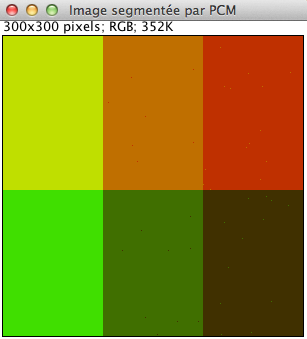
\includegraphics[width=5cm]{images/pcm_img_sup}
	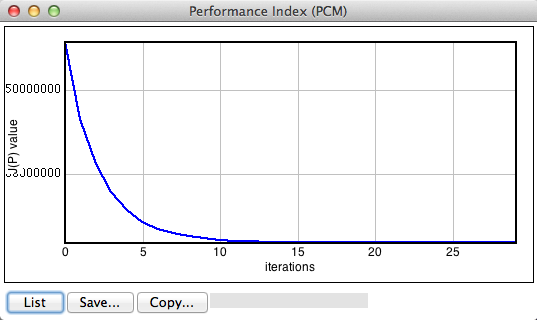
\includegraphics[width=9cm]{images/pcm_courbe_sup}
\end{center}
	\caption{Image r\'esultant de la m\'ethode PCM avec sa courbe de performance}
	\label{}
\end{figure}

\section{Dav\'e}

Enfin pour Dav\'e on reprend le m\^eme principe que PCM \`a une diff\'erence pr\`es. Au lieu d'exclure les points qui ne sont pas repr\'esentatif de la classe (cluster) on va les enlever de cette classe et les mettre dans une nouvelle classe "bruit".

\begin{figure}[ht]
\begin{center}
	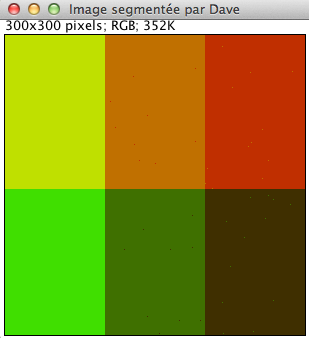
\includegraphics[width=5cm]{images/dave_img_sup}
	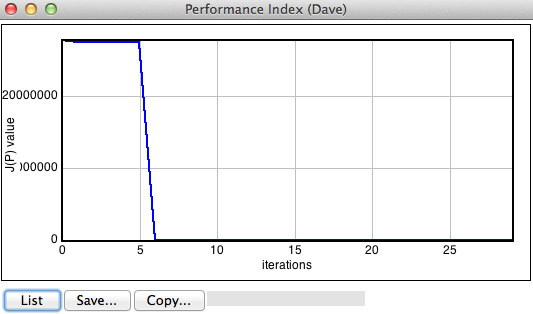
\includegraphics[width=9cm]{images/dave_courbe_sup}
\end{center}
	\caption{Image r\'esultant de la m\'ethode Dav\'e avec sa courbe de performance}
	\label{}
\end{figure}

\newpage

\section{Modification de l'indice de flou pour la m\'ethode FCM}

Voici les r\'esultats obtenu en changeant la valeur de l'indice de flou pour la m\'ethode FCM (les autres valeurs sont les m\^emes).

\begin{figure}[ht]
\begin{center}
	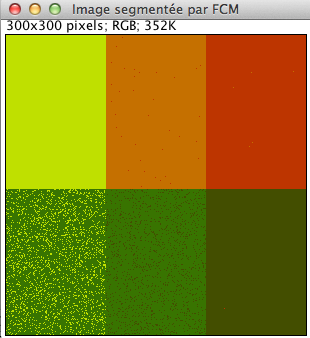
\includegraphics[width=5cm]{images/fcm_img_floue_5}
	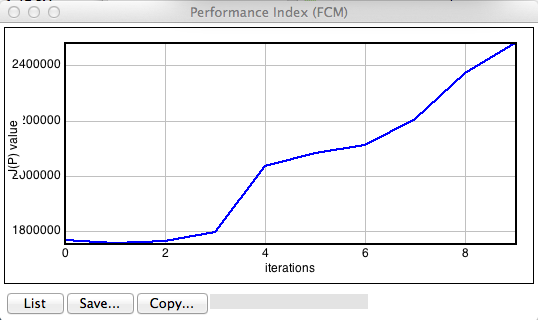
\includegraphics[width=9cm]{images/fcm_graph_floue_5}
\end{center}
	\caption{Image r\'esultant de la m\'ethode FCM avec sa courbe de performance. L'indice de flou vaut 5.}
	\label{}
\end{figure}

\begin{figure}[ht]
\begin{center}
	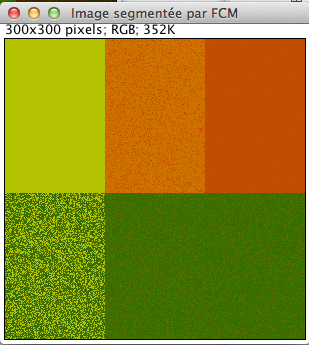
\includegraphics[width=5cm]{images/fcm_img_floue_10}
	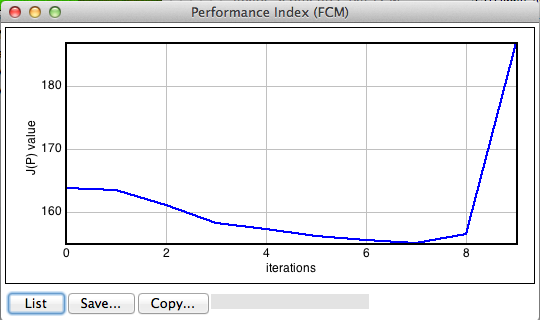
\includegraphics[width=9cm]{images/fcm_graph_floue_10}
\end{center}
	\caption{Image r\'esultant de la m\'ethode FCM avec sa courbe de performance. L'indice de flou vaut 10.}
	\label{}
\end{figure}

\begin{figure}[ht]
\begin{center}
	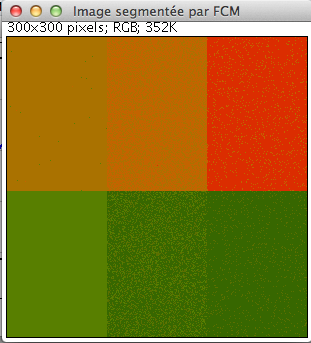
\includegraphics[width=5cm]{images/fcm_img_floue_15}
	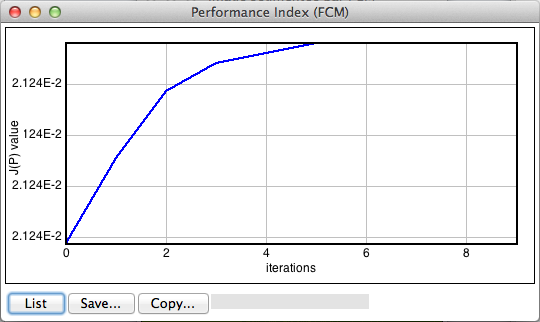
\includegraphics[width=9cm]{images/fcm_graph_floue_15}
\end{center}
	\caption{Image r\'esultant de la m\'ethode FCM avec sa courbe de performance. L'indice de flou vaut 15.}
	\label{}
\end{figure}

\newpage

On voit bien que plus l'indice de flou est grand plus la taille du cluster l'est et donc on observe une fusion des clusters.

\end{document}